\PassOptionsToPackage{utf8}{inputenc}
\documentclass{bioinfo}

\usepackage{makecell}

\usepackage{floatrow}

\usepackage{comment}

\usepackage{siunitx}

% singlelinecheck=false puts subcaptions on the left
\usepackage[singlelinecheck=false]{subcaption}

\usepackage[usenames,dvipsnames]{xcolor}

\usepackage{amsthm}
\theoremstyle{definition}
\newtheorem{definition}{Definition}[section]
\newtheorem{theorem}{Theorem}[section]
\newtheorem{corollary}{Corollary}[theorem]
\newtheorem{lemma}[theorem]{Lemma}

\usepackage{algorithm2e}
\SetKwRepeat{Do}{do}{while}%

% we squeeze our figures even more together
\captionsetup{belowskip=-2pt}

\SetAlgoLined
\SetKwProg{MyStruct}{Struct}{ contains}{end}

\newcommand{\vocab}{\textbf}
\newcommand{\red}[1]{{\textcolor{Red}{#1}}}
\newcommand{\FIXME}[1]{\red{[FIXME: #1]}}

\usepackage{orcidlink}
\hypersetup{hidelinks}


\def\labelitemi{--}

\copyrightyear{2022} \pubyear{XXXX}

\access{Advance Access Publication Date: Day Month Year}
\appnotes{Genome Analysis}

\begin{document}
\firstpage{1}

\subtitle{Genome Analysis}

\title[Wavefront inception]{Whole genome alignment with wavefront inception}
\author[Guarracino \textit{et~al}.]{
Andrea~Guarracino\,$^{\orcidlink{0000-0001-9744-131X}\text{\sfb 1}}$,
Njagi~Mwaniki\,$^{\text{\sfb 2}}$,
Santiago~ Marco-Sola\,$^{\orcidlink{0000-0001-7951-3914}\text{\sfb 3, 4}}$,
Erik~Garrison\,$^{\orcidlink{0000-0003-3821-631X}\text{\sfb 5}*}$
}

\address{
$^{\text{\sf 1}}$Genomics Research Centre, Human Technopole, Viale Rita Levi‑Montalcini 1, Milan, 20157, Italy \\
$^{\text{\sf 2}}$Department of Computer Sciences, University of Pisa, Pisa, 56127, Italy \\
$^{\text{\sf 3}}$Department of Computer Sciences, Barcelona Supercomputing Center, Barcelona, 08034, Spain \\
$^{\text{\sf 4}}$Department d’Arquitectura de Computadors i Sistemes Operatius, Universitat Autònoma de Barcelona, Barcelona, 08193, Spain \\
$^{\text{\sf 5}}$Department of Genetics, Genomics and Informatics, University of Tennessee Health Science Center, Memphis, 38163, Tennessee, USA
}


\corresp{
$^\ast$To whom correspondence should be addressed.
%$^\dagger$Contributed equally.
}

\history{Received on XXXXX; revised on XXXXX; accepted on XXXXX}

\editor{Associate Editor: XXXXXXX}

\abstract{
\textbf{Motivation:}
Pairwise alignment is essential to understanding DNA sequence variation.
The time and memory required to compute pairwise alignments increases quadratically with sequence length and nucleotide divergence.
Advances in sequencing technology have resulted in the rapid production of new whole-genome sequences.
This leads to a new problem of efficiently comparing many whole genomes, a costly task for methods designed to align shorter (100bp--100kbp) sequence reads to reference genomes. \\
%This makes it impractical to align very long sequences without applying heuristic approaches to first determine possible synthenic regions in the sequences.
%Nevertheless, with the advances in sequencing technologies, new whole-genome assemblies are produced at a high rate, pressing for the development of tools able to align sequences of the order of tens of megabases long. \\
\textbf{Results:}
Here we present \textit{wfmash}, a sequence aligner specialized for large collections of very long and highly divergent genome sequences.
It first finds large syntenic homologies between genomes using locality sensitive hashing, approximate match chaining, and logarithmic-time filtering of these mappings.
%Two parameters define these mappings: a seed segment length and minimum average nucleotide identity between matched segments, allowing for intuitive experimental setup.
The resulting mappings can cover entire chromosomes and contain megabase-scale SVs, which presents a significant challenge for direct alignment.
We address this with an extension of the wavefront algorithm (WFA) that matches segments of sequence rather than single characters.
Our approach achieves a many thousand-fold reduction in time and space complexity relative to direct alignment with WFA.
We demonstrate that this comes at little to no cost in terms of variant detection accuracy relative to established sequence aligners. \\
%\textit{wfmash} allows us to scale to all-to-all alignment of hundreds of vertebrate \\
%A key feature of \textit{wfmash} is that users can intuitively shape the scope of an alignment experiment using two parameters: a mapping segment length and a minimum average nucleotide identity between segments. \\
\textbf{Availability:}
wfmash is published as free software under the MIT open source license.
Source code and documentation are available at \url{https://github.com/ekg/wfmash}.
wfmash can be installed via Bioconda \url{https://bioconda.github.io/recipes/wfmash/README.html} or GNU Guix \url{https://github.com/ekg/guix-genomics/blob/master/wfmash.scm}. \\
\textbf{Contact:} \href{egarris5@uthsc.edu}{egarris5@uthsc.edu} \\
%\textbf{Supplementary information:} Supplementary data are available at \textit{Bioinformatics} online.
}

\maketitle

\section{Introduction}
\label{sec:introduction}
Sequence alignment determines edits that transform one sequence into another.
This is a core task in biological analysis, with applications ranging from short read~mapping~\citep{Langmead2012, li2013aligning, MarcoSola2012}, variant detection~\citep{DePristo2011}, to de~novo assembly~\citep{Simpson2009} and pangenome construction~\citep{Armstrong2020, Li2020, pggb}.
Pairwise sequence alignment can be applied to identify similar regions that may indicate functional, structural, and/or evolutionary relationships between two biological sequences.
It is key to our study of evolution.

Due to the intrinsic quadratic difficulty of exact alignment algorithms, and the concomitant need for heuristic algorithms that render them practical, solutions to the problem of sequence alignment are tied closely to the DNA sequence types being considered.
However, the basic concepts behind sequence alignment have not changed in more than 30 years.
Methods like FASTA \citep{Pearson_1988}, BLAST \citep{Altschul_1990}, BLAT \citep{Kent_2002}, and LASTZ \citep{harris2007lastz} focused on high sensitivity alignment driven by short match (e.g. $k$-mer) seeds, chaining and filtering of seeds to find candidate alignments, and final base level alignment using algorithms like Smith-Waterman-Gotoh \citep{Gotoh_1982}.
Short read sequencing led to a deluge of sequencing data that led to a wave of aligners focused on the problem of matching short (100-250bp) reads with few errors to reference genomes of several gigabase-pairs \cite{Langmead2012,MarcoSola2012,li2013aligning}.
These methods employ various full text indexes to speed up match discovery, including the FM-index \citep{Ferragina_2000}, which supports linear-time exact matching queries that are ideal for application to precise alignment of high-accuracy sequence reads.

Increasing sequence read lengths and the arrival of whole genome assemblies for many species rendered such approaches more sensitive than necessary.
Sparsification, or random sampling to reduce computational costs, allows tremendous improvement in performance.
We can still achieve near-perfect alignment performance when mapping long reads to reference genomes even when ignoring many parts of the query and target sequences.
%The new problem of mapping long reads to reference genomes led to 
Methods like minimap2 \citep{Li_2018}, LRA \citep{Ren_2021}, Winnowmap \citep{Jain_2020}, and MashMap \citep{Jain_2018} compute mappings, or candidate alignments, using a sparse subset of all $k$-mers, which are often referred to as ``minimizers'' due to their definition as hash-minimizing $k$-mers in a given window \cite{Roberts_2004}.
Rather than considering all $k$-mers, \textit{windowed minimizer} sampling collects $\sim L/w$ $k-mers$ from a sequence of length $L$, wherein each $k$-mer minimizes a given hash function within a window of size $w$.
This sampling scheme provides guarantees about the distribution of sampled $k$-mers, which aids read alignment and mapping chaining.
It has been discovered that window minimziers are biased and may underestimate the true similarity of sequences \citep{Belbasi_2022}.
In contrast, \textit{world minimizers}, which sparsify over the entire potential space of $k$-mers \citep{Broder_1997}, are not biased, and have proved useful as the basis for the whole genome comparison system Mash \citep{Ondov_2016}.

With the arrival of many whole genome assemblies for vertebrates \citep{Rhie_2021}, as well as the first complete assembly of the human genome \cite{Nurk_2022}, the length of sequences that we seek to align has increased again by several orders of magnitude.
Instead of aligning sequences of 100kb, we now must consider the alignment of whole chromosomes of 100Mbp.
At the same time, the development of pangenomes based on collections of many such genomes (as in the human pangenome project, HPRC) increases the size of a mapping target from 1Gbp to 1Tbp.
This $10^3$-fold increase in scale leads to a new set of problems. % that lead towards our specific contribution in the current work. 
Sequence mappers based on minimizer chaining have mapping costs of $O(n \log n)$ for long sequences \citep{Jain_2022}, where $n$ is the number of seeds.
The vast number of minimizers and minimizer chains found when mapping whole chromosomes into a pangenome causes a dramatic increase in overall runtime, particularly when mapping repetitive sequences that are now accessible using improved 3rd-generation sequencing technology \citep{Logsdon_2021,Nurk_2022}.

%Minimizer seeds have also proven useful for the generation of alignments.
%To obtain base level alignments using adaptive-banded Smith-Waterman-Gotoh requires seeds that initiate the correct alignment, rendering the use of minimizers necessary.
%But, this limits the level of further sparsification available to mapping methods.
%These costs are further exacerbated when obtaining the base level alignments.

\subsection{Current work}

Here we show that, just as with previous leaps in assembly resolution, we can radically improve alignment performance for this new scale by further the degree to which we sparsify, or sample, key information driving mapping and alignment.
We present wfmash, an ultra-scalable sequence aligner for whole genomes and pangenomes.
%Our goals are different: we seek to build alignments that represent synteny across whole chromosomes, and we are less concerned about 
To obtain approximate mappings between pairs of genomes, wfmash extends MashMap \citep{Jain_2018}, which has proven to be the fastest homomoly mapping method, adapting it to use world minimizers, extending it with a new mapping chaining approach designed to find maximal syntenic blocks even in the presence of large structural variants.

However, obtaining a base level alignment required a completely new approach to sequence alignment.
We exploit the $O(s^2)$ scaling properties of the WaveFront Algorithm (WFA) \citep{Marco_Sola_2020} in a new hierarchical arrangement (the ``we flying'' alignment algorithm, WFlign) wherein WFA is applied not to the matching of single characters of input genomes, but rather to the matching of segments of hundreds of base-pairs (e.g. 256bp) (WF$\lambda$).
These segments are matched by sketching their kmers, and where similarity is above a given threshold, an ``incepted'' WFA alignment is completed at the base level.
By taking half-overlapping segments, the method has a high probability of finding the optimal base-level alignment within the incepted WFA problems, and we ultimately combine these during traceback through the WF$\lambda$ matrix.
A final round of erosion and patching of the resulting alignment (with WFA) yields a base-level alignment.

For a segment length $L$, wavefront inception provides $O(4L^2)$ reduction in alignment complexity relative to direct application of WFA.
When $L=256$, this corresponds to a 16,384-fold reduction in computational complexity, a property born out by our experimental results.
Although WFlign is an approximate alignment algorithm not guaranteed to find the optimal alignment through the full matrix, here we show that our implementation nevertheless achieves state-of-the-art accuracy for variant detection via alignment.

%A collection of minimizers of a given length is often referred to as a sketch, and is a form of locality sensitive hash that may be quickly compared to obtain sequence similarity estimates without consideration of the full sequence, as in mash \cite{Ondov_2016}.
%Minimizers have been applied to numerous problems in sequence analysis, but the 
%

\begin{figure}[ht!]
    \begin{subfigure}{\linewidth}
        %\caption{}
        \centering
        % include first image
        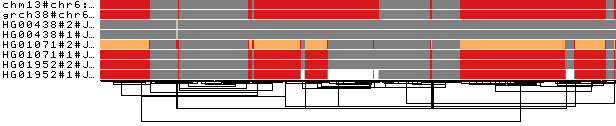
\includegraphics[width=1.0\linewidth, trim=-0cm 2cm 0 0cm]{fig/wflambda/chr6_pan_fa_a2fb268_4030258_6a1ecc2_smooth_C4_bad_sorted}
        \label{fig:bad-sorting}
    \end{subfigure}
%	\includegraphics[width=\linewidth]{fig/metrics/chr4.pan.HTTex1.gfa.multiqc_odgi_stats.png}
    \caption{
        PLACEHOLDER IMAGE XXX XXX XXX
    }
    \label{fig:wflambda}
\end{figure}



\section{Methods}
\label{sec:methods}

wfmash first applies a locality-sensitive hashing, from MashMap, to rapidly determine syntenic region boundaries between long DNA sequences.
Then, a hierarchical implementation of the WFA allows computing the base-level global alignment of the identified mappings.

\subsection{Approximate mapping}
Each query sequence is broken into non-overlapping pieces of the requested length.
These segments are then mapped using MashMap's sliding MinHash mapping algorithm~\citep{Jain_2018}.
We extended MashMap by incorporating the robust winnowing~\citep{Schleimer2003} in the minimizer sampling.
Robust sampling avoids taking too many minimizers in low-complexity regions in the sequences, yielding improvements in runtime and memory-usage without affecting accuracy~\citep{Jain_2020}.
Furthermore, we made it possible to set the number of mappings to return for each segment; this is useful for identifying paralogous regions and homologous relationship between sets of genomes.
Together with the segment length and the minimum segment estimated identity, these settings allow users to precisely define the mapping space to consider, specifying the characteristics of homologies to compute.
%TODO THINGS ON THE FILTERING???
%TODO THING ON THE SPLIT READ AND/OR THE MERGING???

\FIXME{World minimizers XXXXXX}

\FIXME{Spaced-seed XXXXXX}


\subsection{Base-level alignment with wflambda}
Each mapping location is used as a target for base-level alignment using a hierarchical implementation of the WFA.
Time and space computational complexities of a base-level alignment are quadratic with respect to the sequence length.
The WFA provides an efficient way to decrease the amount of computation required to obtain the optimal alignment between two sequences, reducing the computational cost to be quadratic in the alignment penalty score of the optimal alignment~\citep{Marco_Sola_2020}.
This means that WFA is very efficient in aligning similar homologous sequences (i.e., sequences with a low alignment penalty score), but high divergence genomes and/or noisy long reads can increase its time and memory costs.

To avoid such limitation, wfmash applies a hierarchical WFA, exploiting the WFA to guide the alignment process, but keeping the largest alignment problem size small.
Rather than directly aligning the whole sequences, it aligns them to each other in small pieces \textit{W}-bp long by applying a global WFA alignment (Figure~1\vphantom{\ref{fig:1}}).
The whole global alignment is then computed over the full dynamic-programming matrix (high order DP-matrix) at \textit{W}-bp resolution.
Each cell in the high order DP-matrix corresponds to the alignment of a specific pair of fragments \textit{W}-bp long from the two sequences to align.

\subsection{Sparsification}
To determine if each cell is a match, and then guiding the alignment at \textit{W}-bp resolution, the global alignment is performed between the two fragments with the standard WFA.
To accelerate the process, an alignment-free comparison of the two fragments is performed first by computing the mash distance between them.
Cells whose fragments have a high mash distance are considered as mismatches, avoiding computing the corresponding base-level alignments.

\subsection{Patching}
Finally, the \textit{W}-bp resolution traceback is applied to determine the set of base-level alignments on the optimal path in the high order DP-matrix.
During the process, a further step is performed for refining the alignment.
Inaccurate mapping estimation can lead to under-alignment at the beginning and the end of the aligned syntenic region.
Therefore, WFA is applied by computing semi-global alignments to resolve the mapping boundaries.
Moreover, the standard WFA is applied to resolve breakpoints of the structural variants when present in the aligned region.

\subsection{Complexity}
The hierarchical implementation requires only the memory to align the sequences at \textit{W}-bp resolution, limiting the runtime and the memory of the standard WFA by applying it to fragments \textit{W}-bp long.
This approach is more \FIXME{flexible than using a fixed-width band (it effectively has a variable bandwidth), requires no heuristic seeding step}, and can benefit from parallel exploration of the wavefront.
%TODO 'this approach is more flexible than using a fixed-width band: Not sure about writing it. I would remove it, else we should demonstrate it.
\\

\section{Results}
\label{sec:results}

\subsection{Input and output features}
XXXXXXXXXXXXX -s, -l, -p, -n, -i, sam/paf

\subsection{Liftover completeness}
XXXXXXXXXXXXXXXXXXXXXXX

\subsection{Pangenome building and evaluation}
We evaluated the performance of wfmash \texttt{90ea671} against Minimap2-v2.20-r1061~\citep{Li_2018} and Winnomap 2.03~\citep{Jain_2020b}, in terms of runtime and memory usage.
The comparison was performed on both simulated and real datasets. Simulated data allowed evaluating the alignment quality by calculating precision and recall in variant identification.
The evaluations were performed on a workstation running \FIXME{Ubuntu 20.04 equipped with 64 GB of RAM and an Intel i9-9900K CPU with 8 cores (16 threads)}.

We simulated long sequences from \FIXME{the \textit{Saccharomyces cerevisiae} chromosome IV (S288C strain) and the telomere-to-telomere (T2T) assemblies of the human chromosomes 8}, at different levels of length and divergence (\FIXME{MAYBETable 1 and Table 2}).
Chromosomes were split into shorter sequences using the splitfa tool (6a0bb67)~\citep{splitfa-gh}.
In each run, all sequences have the same length, with half of them in reverse complement respect to the source chromosome.
Single nucleotide variants~(SNVs), small indels, and structural variants~(SVs) were introduced using the Mutation-Simulator script~\citep{Khl2020}.
\FIXME{Structural variants (SVs) were applied using the SURVIVOR benchmarking tool}~\citep{Jeffares2017}.

To evaluate the correctness of the alignments, we used the pairwise alignment of the input sequences from each run to build a pangenome graph and identified the variants embedded in it.
The graphs were built with seqwish~\citep{Garrison2022}, a lossless pangenome graph inducer.
We called SNVs, small indels, and SVs using vg deconstruct~\citep{Garrison:2018}, evaluating the false-negative and false-positive rates using vcfeval~\citep{Cleary2015} for SNVs and small indels, and \FIXME{XXXXX for SVs}.


\subsection{Pangenome alignment (ONT vs HPRC)}
XXXXXXXXXXXXX


\begin{comment}

\begin{table}[!t]
    \processtable{
        \small
        Performance of pairwise alignment of long sequences from the \textit{Saccharomyces cerevisiae}
        chromosome IV.
        \label{Tab:01}} {
        \begin{tabular}{@{}llllllll@{}}
            \toprule Aligner & Divergence & Length & Runtime (mm:ss) & Memory (GB) & Precision & Sensitivity & F-measure \\
            \midrule
            row1             & row1       & row1   & row1            & row1        & row1      & row1        & row1      \\
            row2             & row2       & row2   & row2            & row1        & row1      & row1        & row1      \\
            row3             & row3       & row3   & row3            & row1        & row1      & row1        & row1      \\
            row4             & row4       & row4   & row4            & row1        & row1      & row1        & row1      \\
            \botrule
        \end{tabular}
    }
\end{table}


\subsection{Real data}
\\
% Yeast/HPRC data time/memory
% Histogram of the contig length distribution (supplementary?)


\end{comment}


\section{Discussion}
\label{sec:discussion}

We implemented a novel gap-affine pairwise aligner, wfmash, to accelerate the computation of the mutual alignment of collections of genomes, a step required for constructing pangenome models.
We have demonstrated that it efficiently performs with contigs representing full human chromosomes of 88 phased haplotypes from the Human Pangenome Reference Consortium year 1 assembly.
Indeed, thanks to its efficiency, wfmash is already successfully applied in our pangenome graphs building pipeline~\citep{pggb}.
No less important, pairwise alignment is a central step of many bioinformatics applications, making our aligner a scalable solution to face the increasing yields of sequencing technologies in the coming years.


\subsection{Limits and potential improvements}

XXXXX

\section*{Acknowledgements}

We thank members of the HPRC Pangenome Working Group for their insightful discussion and feedback, and members of the HPRC production teams for their development of resources used in our exposition.
%todo VGP/EBP too?

\section*{Funding}

We gratefully acknowledge support from NIH/NIDA U01DA047638 (EG) and efforts by Dr. Nicole Soranzo to establish a pangenome research unit at the Human Technopole in Milan, Italy (AG).
\linebreak
\linebreak
\textit{Conflict of Interest}: none declared.

\section*{Data availability}

Code and links to data resources used to build this manuscript and its figures can be found in the paper's public repository: \url{https://github.com/AndreaGuarracino/wfmash-paper}.

\bibliographystyle{natbib}

\bibliography{document}

\end{document}
